\chapter{Investigation by Simulation}

\textcolor{blue}{
\begin{itemize}
    \item Simulated Microgrid
    \item Simulation of "accurate" interconnection model for 1-2 seconds using SPWM
    \item Simulation of "accurate" interconnection model for 1-2 seconds using SVPWM
    \item Simulation of averaged model of interconnection for longer durations (e.g., 1 minute)
    \item Simulation to demonstrate transfer of poweR 
\end{itemize}
}

\section{Model Simulation}

As has been described, the intent of this project is to form an interconnection via which two microgrid- and nanogrid-scale power systems can exchange power as needed. It is critical to identify key characteristics of these power systems.

\subsection{Three-Phase SRF-PLL}

For the purposes of this experiment, it has been decided that a phase-locked loop is to be used for synchronization; that is because it has a greater ability to withstand distortions within the input signal and disturbances at the output \cite{Guerrero_Vasquez_3PLL}.

A key component of the synchronizing module, the three-phase SRF-PLL, is modeled in \textsc{MATLAB}. To verify its ability to track a changing reference frequency, its response to the example input signal 
\begin{equation}
    u(t) = \sin(2{\pi}ft)
\end{equation}
is simulated. The value of $f$ in this signal varies from 60 Hz to 65 Hz.
\begin{comment}
\begin{figure}
    \centering
    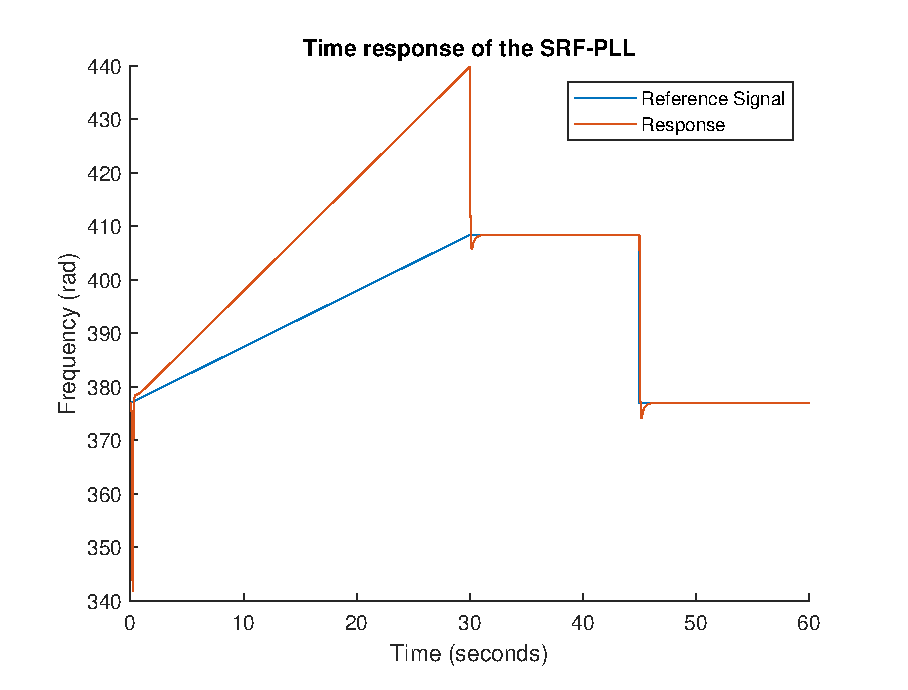
\includegraphics[width=0.75\linewidth]{Images/Sine_variation_Graph_Real.eps}
    \caption{The response of the simulated SRF-PLL}
    \label{fig:SRFPLL_Fig1}
\end{figure}
\end{comment}
The response is graphed in \autoref{fig:SRFPLL_Fig1}, The results show that, while the SRF-PLL cannot track a ramp signal without steady-state error, it is able to track a constant signal.

To test the PLL's response within the context of a power system, its performance in measuring an inverter's output frequency is tested. The simulation environment within MATLAB is shown in \autoref{fig:SimInverter}. The inverter is powered by a DC voltage source at 208 $V$. The PLL has proportional gain $k_p = 2$ and integral gain $k_i = 1000$. The reference signal is

\begin{equation*}
    \textbf{u}(t) = 
        \begin{bmatrix}
            120\sin(377t) \\
            120\sin(377t - \frac{2\pi}{3}) \\
            120\sin(377t - \frac{4\pi}{3})
        \end{bmatrix} \mathrm{V}
\end{equation*}

which is a three-phase signal with frequency of 60 Hz. It assumed to come from an infinite bus. 

\begin{figure}
    \centering
    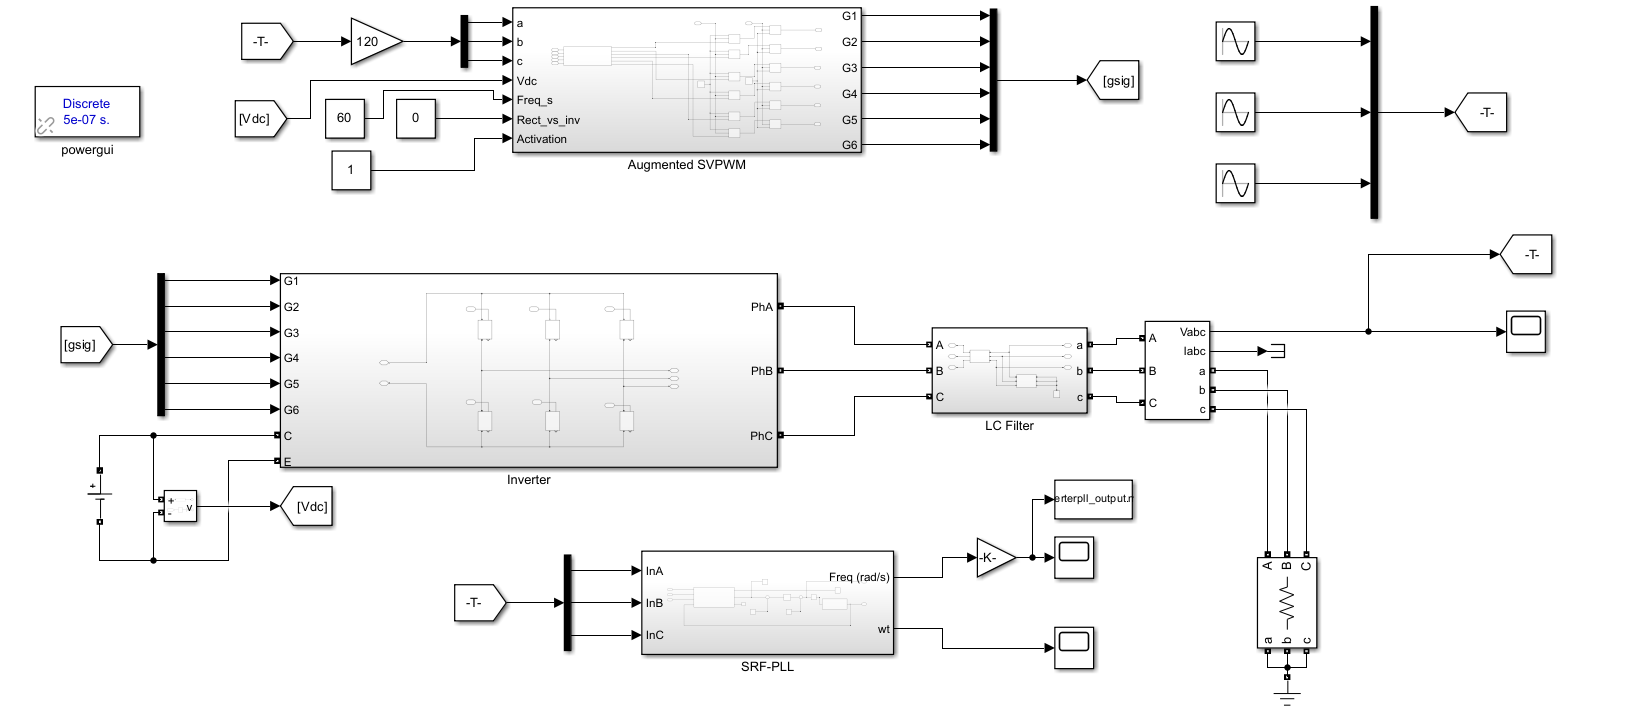
\includegraphics[width=\linewidth]{Images/MATLAB System.png}
    \caption{Simulated Inverter}
    \label{fig:SimInverter}
\end{figure}

The graph in \autoref{fig:SimInverter_Frequencies} shows that, while there is substantial overshoot, the response is extremely rapid, settling to its final value of 60 Hz in less than 0.2 s. This suggests that the designed PLL can track changes in reference frequencies, but it may risk reacting too quickly to noise from a reference signal.

\begin{figure}
    \centering
    \includegraphics[width=0.95\linewidth]{Images/Frequencies.eps}
    \caption{Output Frequencies of Simulated Inverter}
    \label{fig:SimInverter_Frequencies}
\end{figure}

\subsection{Model of the "Weak" Power Systems}

\subsection{Model of a Power Electronic Based Bidirectional Converter}

As a baseline, an AC-AC converter with a DC link is simulated. The AC-AC converter is composed of two six-switch converters (i.e., a rectifier and an inverter) in cascade. In simulation, the terminals of both six-switch converters are connected to a three-phase voltage source and a three-phase load, respectively, to evaluate whether both terminals could serve in each capacity. Furthermore, to ensure that both terminals can service power sources and/or loads that are serving at different frequencies, each terminal is tested with a 60 Hz power source and a 50 Hz load. The results are plotted below. It can be seen that, on both ends, the desired frequencies are obtained.

\begin{figure}[h]
    \centering
    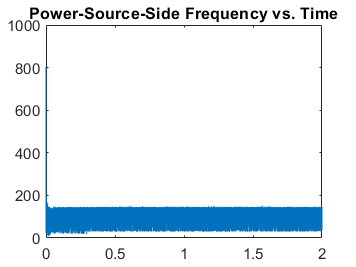
\includegraphics[width=0.6\linewidth]{Images/IMG_0994.png}
    \caption{Frequency of Power Source in Simulated AC-AC Converter}
    \label{fig:Investigations_60Hz}
\end{figure}

The image in \autoref{fig:Investigations_60Hz} shows the frequency of the input fixed voltage source. It is 60 Hz. Meanwhile, the image in \autoref{fig:Investigations_50Hz} shows the frequency at the load-side terminal. It is 50 Hz.

\begin{figure}[h]
    \centering
    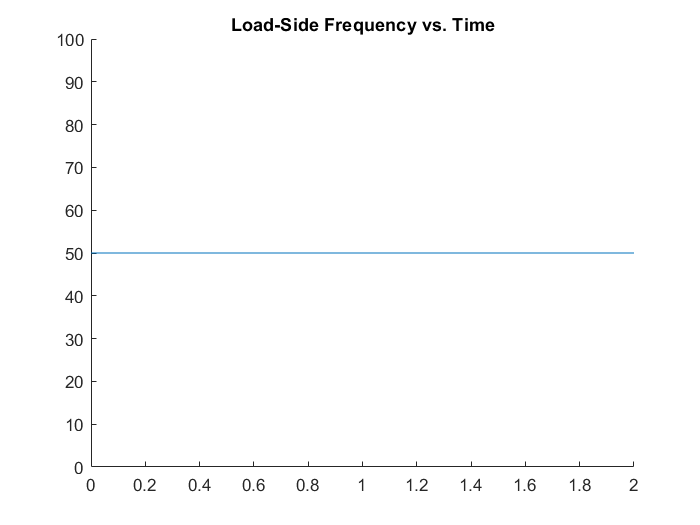
\includegraphics[width=0.6\linewidth]{Images/IMG_0995.png}
    \caption{Frequency at Load Side in Simulated AC-AC Converter}
    \label{fig:Investigations_50Hz}
\end{figure}

% Add diagram

% \section{Connection Transients \& Dynamic Interactions}

\section{Alternative Modulation Schemes}

The inverter is tested using both sinusoidal pulsed width modulation (SPWM) and space vector pulsed width modulation (SVPWM). 